\subsection{Role Based Access Control}
\label{sec:rbac}

Diese Pattern basiert stark auf dem Authorization Pattern und versucht dessen Nachteile durch einen zusätzlichen Abstraktionslayer auszugleichen.
Das ''Role Based Access Control'' Pattern definiert Berechtigungen nicht direkt auf Stufe der Subjekte, sondern versucht diese in Gruppen (Aufgabenbereiche, Kaderposition, Arbeitsort etc.) einzuteilen und anschliessend auf dieser Ebene quasi übergeordnet zu berechtigen.

\subsection*{Kontext}
Eine Umgebung mit vielen Objekten und Subjekten. Deren Berechtigungen ändern häufig. Zudem ist damit zu rechnen dass eben so oft neue Subjekte und Objekte hinzukommen oder wieder wegfallen.

\subsection*{Problem}
Die Rechteverwaltung in dem beschriebenen Kontext generiert einen hohen administrativen Aufwand. Um die Anzahl individueller Berechtigungen zu minimieren soll versucht werden, alle Subjekte in Gruppen einzuteilen. Die Einteilung basiert darauf, dass Subjekte mit ähnlichen Aufgaben zumeist auch ähnliche oder identische Berechtigungen benötigen.
Trotzdem sollen die Berechtigungen weiterhin präzise abgebildet werden können (''Need to know'').

\subsection*{Lösung}
Organisationen bieten normalerweise bereits mehr oder weniger wohldefinierte Gruppenstrukturen (Abteilungen, Aufgabenbereiche).
Ein gutes Sicherheitskonzept sollte bestrebt sein, dass jedes Subjekt genau auf die Objekte Zugriff hat, mit welchen es täglich arbeitet (wiederum ''Need to know'').

\begin{figure}[H]
	\begin{center}
	\begin{tikzpicture}
		\umlclass[x=0,y=0]{User}{id\\name}{}
		\umlclass[x=5,y=0]{Role}{id\\name}{}
		\umlclass[x=12,y=0]{ProtectionObject}{id\\name}{}
		\umlassoc[name=userrole,arg1=memberOf,mult1=*,mult2=*,align1=left,align2=right,pos1=0.1,pos2=0.9]{User}{Role}
		\umlassoc[name=roleobject,mult1=*,attr2=isAuthorizedFor|*,align1=left,align2=right,pos1=0.1,pos2=0.9]{Role}{ProtectionObject}
		\umlassocclass[geometry=|-|,x=7,y=-2.8]{Right}{roleobject-1}{accessType}{checkRights()}
	\end{tikzpicture}
	\end{center}
	\caption{Basic Role Based Access Control Klassendiagramm}
\end{figure}

Im Vergleich zum Authorization Pattern kommt lediglich ein neues Element hinzu: Die Role fasst mehrere User (Subjekte) zu einer Menge zusammen und berechtigt sie über Right für ein spezifisches ProtectionObject.


\subsection*{Erweiterungen}
\begin{figure}[H]
	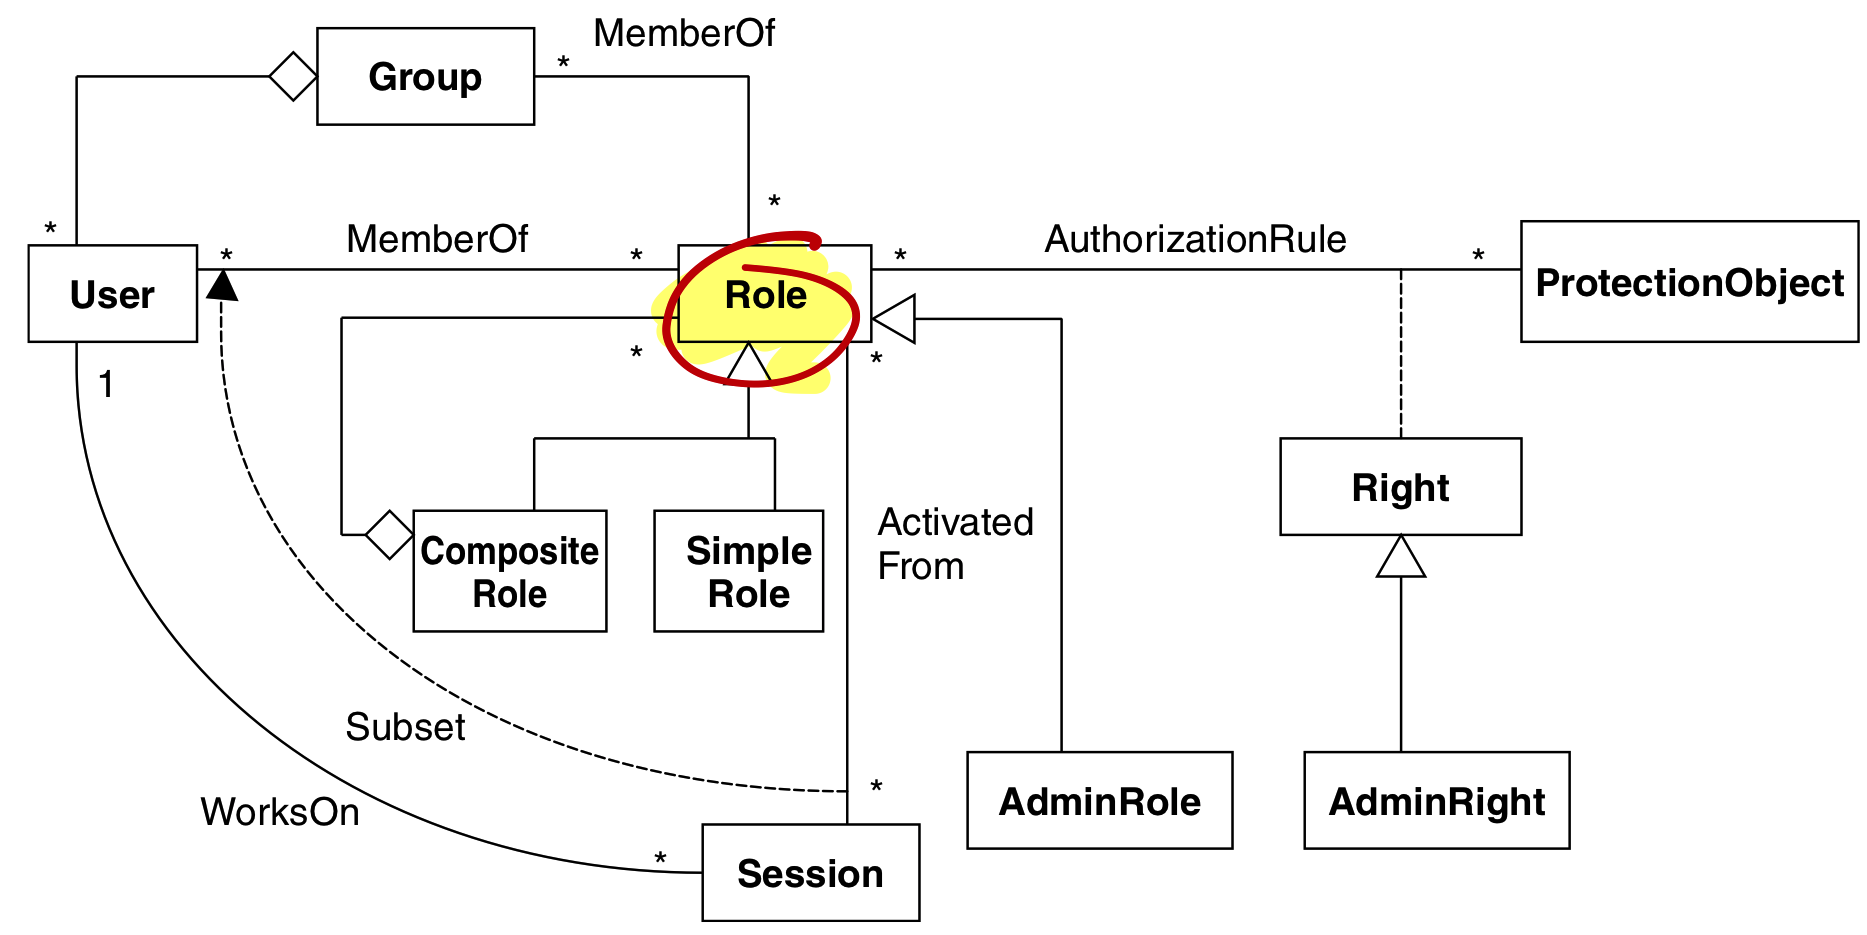
\includegraphics[width=\textwidth]{content/security/accesscontrolmodels/images/rolebasedaccesscontroladvanced.png}
	\caption{RBAC mit Composite, Admins \& Abstract Session}
\end{figure}

\subsubsection*{Composite Pattern}
Statt einer simplen Assoziation zwischen User und Role könnte auch mit dem Composite-Pattern gearbeitet werden, um diese Abhängigkeit zu modellieren.

\subsubsection*{Administration}
Wie ebenfalls bereits im Authorization-Pattern erwähnt kann auch dieses Modell zielgerichtet um Administrations-Elemente erweitert werden.
Auf diese Weise kann zusätzliche Klarheit im System geschaffen werden, wer genau für was zuständig ist.

\subsubsection*{Abstract Session}
Um die Möglichkeiten auf die Spitze zu treiben, sei hier auch das Abstract Session Pattern erwähnt: Die Abhängigkeit einer Session kann so direkt ins Security Modell ''miteinmodelliert'' werden.

\subsection*{Vor- \& Nachteile}
\begin{itemize}
	\item Die Zusammenfassung zu Gruppen ermöglicht eine vereinfachte Administration der gesamthaft vorhandenen Berechtigungen
	\item Veränderungen in der realen Organistaionstruktur (Neuzugänge, Abgänge, Jobwechsel etc.) können einfacher auf das Sicherheitskonzept abgebildet werden
	\item Ein Subjekt kann durch mehrere Sessions verschiedene Funktionen auf einmal wahrnehmen
	\item Theoretisch können Gruppen wiederum in Gruppen zusammengefasst werden (Yay, even more complexity...)
	\item Konzeptionelle Komplexität nimmt durch die neuen Elemente wiederum zu!
\end{itemize}

\subsection*{Beispielanwendungen}
\begin{itemize}
	\item Windows 2000 Rights Management (Group Policies)
\end{itemize}


\subsection*{Mögliche Prüfungsfragen}
\begin{itemize}
	\item \emph{Ein Subjekt hat die Rollen ``Personalabteilung'' und ``USB Datenaustausch'' zugwiesen. Wie kann verhindert werden, dass das Subjekt Personalinformationen auf einen USB-Stick speichern kann?}\\
	Durch die Implementierung des \emph{Abstract Session} Patterns kann das Subjekt gezwungen werden, sich jeweils nur mit einer bestimmten Rolle am System anzumelden. So hat es jeweils entweder nur auf die Personaldatan zugriff oder kann nur Dateien mit einem USB-Stick austauschen.\\
	\emph{wackeliges Beispiel ;-)}
\end{itemize}